\documentclass{standalone}
\usepackage{tikz}
\usetikzlibrary{patterns, positioning}

\begin{document}
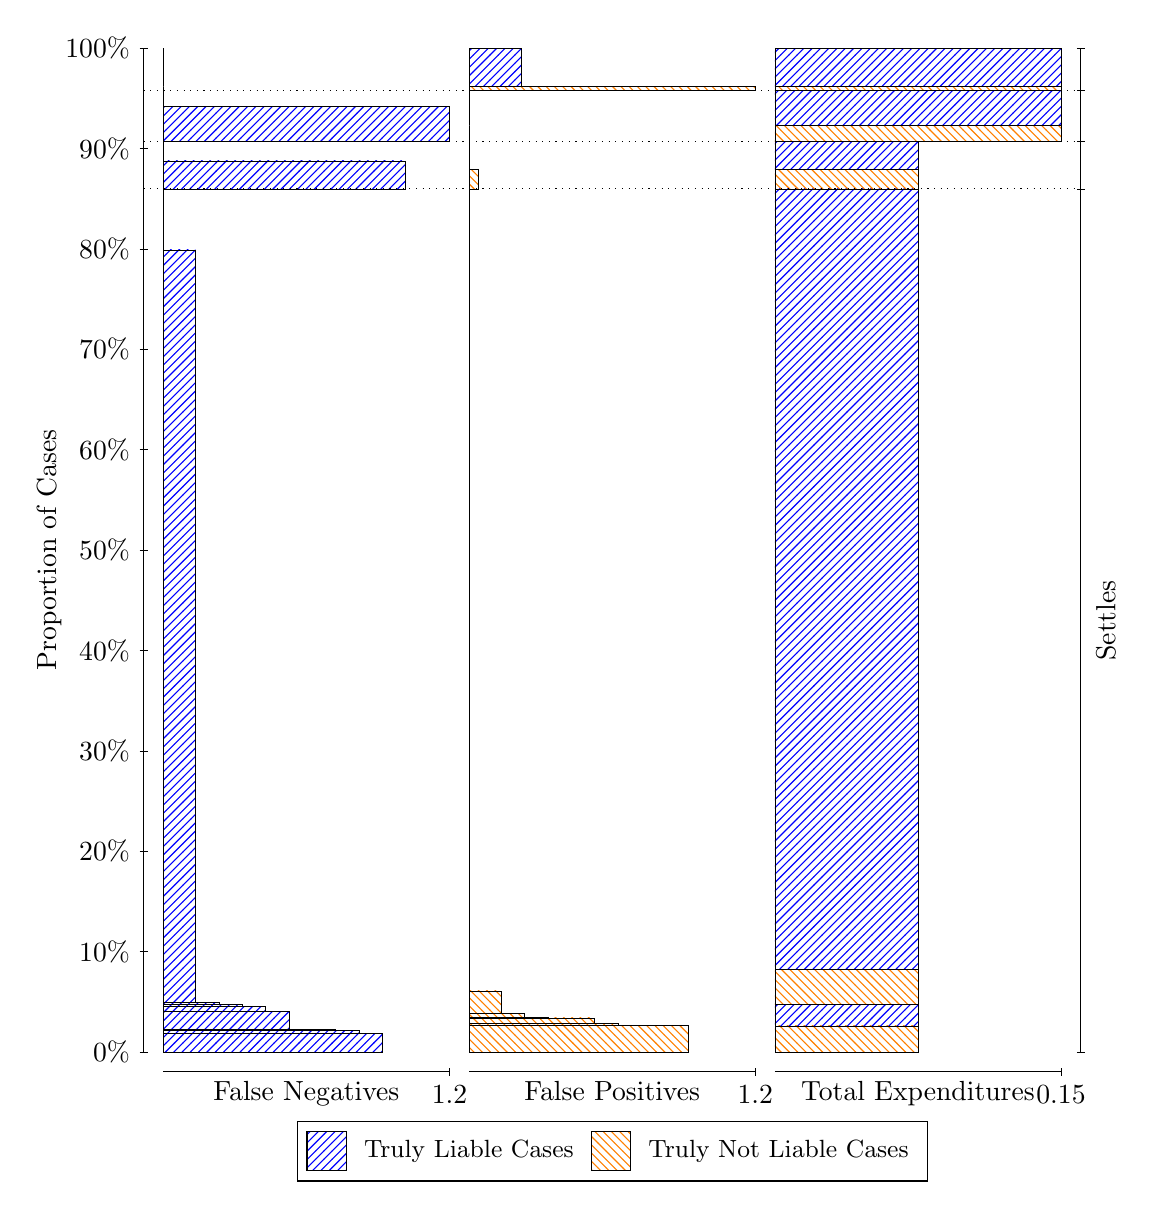
\begin{tikzpicture}
\draw[black, very thin] (1.5,1.75) -- (1.5,14.5);
\node[rotate=90, anchor=center] at (0.3, 8.125) {Proportion of Cases};
\draw[black, very thin] (1.45,1.75) -- (1.55,1.75);
\node[anchor=east] at (1.45, 1.75) {0\%};
\draw[black, very thin] (1.45,3.025) -- (1.55,3.025);
\node[anchor=east] at (1.45, 3.025) {10\%};
\draw[black, very thin] (1.45,4.3) -- (1.55,4.3);
\node[anchor=east] at (1.45, 4.3) {20\%};
\draw[black, very thin] (1.45,5.575) -- (1.55,5.575);
\node[anchor=east] at (1.45, 5.575) {30\%};
\draw[black, very thin] (1.45,6.85) -- (1.55,6.85);
\node[anchor=east] at (1.45, 6.85) {40\%};
\draw[black, very thin] (1.45,8.125) -- (1.55,8.125);
\node[anchor=east] at (1.45, 8.125) {50\%};
\draw[black, very thin] (1.45,9.4) -- (1.55,9.4);
\node[anchor=east] at (1.45, 9.4) {60\%};
\draw[black, very thin] (1.45,10.675) -- (1.55,10.675);
\node[anchor=east] at (1.45, 10.675) {70\%};
\draw[black, very thin] (1.45,11.95) -- (1.55,11.95);
\node[anchor=east] at (1.45, 11.95) {80\%};
\draw[black, very thin] (1.45,13.225) -- (1.55,13.225);
\node[anchor=east] at (1.45, 13.225) {90\%};
\draw[black, very thin] (1.45,14.5) -- (1.55,14.5);
\node[anchor=east] at (1.45, 14.5) {100\%};

\draw[black, very thin] (13.4,1.75) -- (13.4,14.5);
\draw[black, very thin] (13.35,1.75) -- (13.45,1.75);
\node[anchor=west] at (13.35, 1.75) {};
\draw[black, very thin] (13.35,12.712) -- (13.45,12.712);
\node[anchor=west] at (13.35, 12.712) {};
\draw[black, very thin] (13.35,13.317) -- (13.45,13.317);
\node[anchor=west] at (13.35, 13.317) {};
\draw[black, very thin] (13.35,13.964) -- (13.45,13.964);
\node[anchor=west] at (13.35, 13.964) {};
\draw[black, very thin] (13.35,14.5) -- (13.45,14.5);
\node[anchor=west] at (13.35, 14.5) {};

\draw[black, very thin, pattern color=blue, pattern=north east lines] (1.75,1.75) rectangle (4.5306,1.9868);
\draw[black, very thin, pattern color=blue, pattern=north east lines] (1.75,1.9868) rectangle (4.234,2.0263);
\draw[black, very thin, pattern color=blue, pattern=north east lines] (1.75,2.0263) rectangle (3.9374,2.0354);
\draw[black, very thin, pattern color=blue, pattern=north east lines] (1.75,2.0354) rectangle (3.3442,2.2619);
\draw[black, very thin, pattern color=blue, pattern=north east lines] (1.75,2.2619) rectangle (3.0476,2.3281);
\draw[black, very thin, pattern color=blue, pattern=north east lines] (1.75,2.3281) rectangle (2.751,2.3539);
\draw[black, very thin, pattern color=blue, pattern=north east lines] (1.75,2.3539) rectangle (2.4544,2.3803);
\draw[black, very thin, pattern color=blue, pattern=north east lines] (1.75,2.3803) rectangle (2.1578,11.936);
\draw[black, very thin, pattern color=orange, pattern=north west lines] (1.75,11.936) rectangle (1.75,12.712);
\draw[black, very thin, pattern color=blue, pattern=north east lines] (1.75,12.712) rectangle (4.8272,13.068);
\draw[black, very thin, pattern color=orange, pattern=north west lines] (1.75,13.068) rectangle (1.75,13.317);
\draw[black, very thin, pattern color=blue, pattern=north east lines] (1.75,13.317) rectangle (5.3833,13.763);
\draw[black, very thin, pattern color=orange, pattern=north west lines] (1.75,13.763) rectangle (1.75,13.964);
\draw[black, very thin, pattern color=orange, pattern=north west lines] (1.75,13.964) rectangle (1.75,14.012);
\draw[black, very thin, pattern color=blue, pattern=north east lines] (1.75,14.012) rectangle (1.75,14.5);
\draw[black, very thin, pattern color=orange, pattern=north west lines] (5.6333,1.75) rectangle (8.4139,2.0828);
\draw[black, very thin, pattern color=orange, pattern=north west lines] (5.6333,2.0828) rectangle (8.1173,2.0872);
\draw[black, very thin, pattern color=orange, pattern=north west lines] (5.6333,2.0872) rectangle (7.8207,2.0914);
\draw[black, very thin, pattern color=orange, pattern=north west lines] (5.6333,2.0914) rectangle (7.5241,2.1087);
\draw[black, very thin, pattern color=orange, pattern=north west lines] (5.6333,2.1087) rectangle (7.2276,2.1838);
\draw[black, very thin, pattern color=orange, pattern=north west lines] (5.6333,2.1838) rectangle (6.6344,2.1935);
\draw[black, very thin, pattern color=orange, pattern=north west lines] (5.6333,2.1935) rectangle (6.3378,2.241);
\draw[black, very thin, pattern color=orange, pattern=north west lines] (5.6333,2.241) rectangle (6.0412,2.5258);
\draw[black, very thin, pattern color=blue, pattern=north east lines] (5.6333,2.5258) rectangle (5.6333,12.712);
\draw[black, very thin, pattern color=orange, pattern=north west lines] (5.6333,12.712) rectangle (5.7446,12.962);
\draw[black, very thin, pattern color=blue, pattern=north east lines] (5.6333,12.962) rectangle (5.6333,13.317);
\draw[black, very thin, pattern color=orange, pattern=north west lines] (5.6333,13.317) rectangle (5.6333,13.518);
\draw[black, very thin, pattern color=blue, pattern=north east lines] (5.6333,13.518) rectangle (5.6333,13.964);
\draw[black, very thin, pattern color=orange, pattern=north west lines] (5.6333,13.964) rectangle (9.2667,14.012);
\draw[black, very thin, pattern color=blue, pattern=north east lines] (5.6333,14.012) rectangle (6.3007,14.5);
\draw[black, very thin, pattern color=orange, pattern=north west lines] (9.5167,1.75) rectangle (11.333,2.0823);
\draw[black, very thin, pattern color=blue, pattern=north east lines] (9.5167,2.0823) rectangle (11.333,2.3586);
\draw[black, very thin, pattern color=orange, pattern=north west lines] (9.5167,2.3586) rectangle (11.333,2.8021);
\draw[black, very thin, pattern color=blue, pattern=north east lines] (9.5167,2.8021) rectangle (11.333,12.712);
\draw[black, very thin, pattern color=orange, pattern=north west lines] (9.5167,12.712) rectangle (11.333,12.962);
\draw[black, very thin, pattern color=blue, pattern=north east lines] (9.5167,12.962) rectangle (11.333,13.317);
\draw[black, very thin, pattern color=orange, pattern=north west lines] (9.5167,13.317) rectangle (13.15,13.518);
\draw[black, very thin, pattern color=blue, pattern=north east lines] (9.5167,13.518) rectangle (13.15,13.964);
\draw[black, very thin, pattern color=orange, pattern=north west lines] (9.5167,13.964) rectangle (13.15,14.012);
\draw[black, very thin, pattern color=blue, pattern=north east lines] (9.5167,14.012) rectangle (13.15,14.5);
\draw[black, dotted] (1.5,12.712) -- (13.4,12.712);
\draw[black, dotted] (1.5,13.317) -- (13.4,13.317);
\draw[black, dotted] (1.5,13.964) -- (13.4,13.964);
\draw[black, very thin] (1.75,1.5) -- (5.3833,1.5);
\node[anchor=north] at (3.5667, 1.5) {False Negatives};
\draw[black, very thin] (5.3833,1.45) -- (5.3833,1.55);
\node[anchor=north] at (5.3833, 1.45) {1.2};

\draw[black, very thin] (5.6333,1.5) -- (9.2667,1.5);
\node[anchor=north] at (7.45, 1.5) {False Positives};
\draw[black, very thin] (9.2667,1.45) -- (9.2667,1.55);
\node[anchor=north] at (9.2667, 1.45) {1.2};

\draw[black, very thin] (9.5167,1.5) -- (13.15,1.5);
\node[anchor=north] at (11.333, 1.5) {Total Expenditures};
\draw[black, very thin] (13.15,1.45) -- (13.15,1.55);
\node[anchor=north] at (13.15, 1.45) {0.15};

\node[black, centered, rotate=90] at (13.72, 7.2311) {Settles};




\draw (7.449999999999999,1.5) node[draw=none] (baseCoordinate) {};
\begin{scope}[align=center]
        \matrix[scale=0.5, draw=black, below=0.5cm of baseCoordinate, nodes={draw}, column sep=0.1cm]{
            \node[rectangle, draw, minimum width=0.5cm, minimum height=0.5cm, pattern=north east lines, pattern color=blue] {}; &
            \node[draw=none, font=\small] (B) {Truly Liable Cases}; &
            \node[rectangle, draw, minimum width=0.5cm, minimum height=0.5cm, pattern=north west lines, pattern color=orange] {}; &
            \node[draw=none, font=\small] (B) {Truly Not Liable Cases}; \\
            };
\end{scope}

\end{tikzpicture}
\end{document}